\section{Schlussteil}

\subsection{Ausblick}
Es konnte bereits während des Projektes ein gutes Ergebnis erzielt
werden. Dennoch wurden aufgrund der knappen Zeit nicht alle Ideen
umgesetzt. Weitere Möglichkeiten sehen wir im Bereich der nicht
verwendeten Daten und der Nutzung eines Offline-Learning-Verfahrens.
Des Weiteren besteht die Möglichkeit, die verwendeten Features auf ihre
Aussagekraft beziehungsweise Qualität zu untersuchen.

\subsubsection{Verwendung aller Daten}
Es werden bisher hauptsächlich Transaktionen berücksichtigt, die in Beziehung zu Gutscheinen stehen.
Bei diesen Transaktionen muss die Marke, die Kategorie oder das Unternehmen mit dem entsprechenden Gutschein übereinstimmen.
Diese Daten könnten in einem nächsten Iterationsschritt ebenfalls verwertet werden, wozu zunächst die folgenden Ansätze zusammengetragen wurden:
	
\begin{itemize}
\item Für jeden Kunden soll der komplette Umsatz pro Quartal bzw. pro Jahr ermittelt werden. Die Idee ist, dass der Umsatz das Kaufverhalten der Kunden beeinflusst.
 
\item Kunden, die in regelmäßigen Abständen einkaufen, kommen sehr wahrscheinlich wieder.
Beispielsweise werden wöchentlich die Nahrungsvorräte auf dem Heimweg von der Arbeit aufgefüllt.
Die Frequenz des Einkaufens kann über die Auswertung der Zeitangaben der Transaktionen ermittelt werden.

\item Clustering von oft zusammengekauften Marken, Kategorien und Unternehmen
ermöglicht weitere Features für die Kunden zu definieren.
Dies erfordert allerdings die Implementierung eines Clustering-Algorithmus
auf den Daten.
\end{itemize}

\subsubsection{Bewertung von Features}	
Sowohl bei den verwendeten Features als auch bei den oben vorgestellten Ideen ist bisher unklar, inwiefern diese Features das Kaufverhalten positiv, negativ oder überhaupt beeinflussen.
In unseren Vorträgen zur Veranstaltung ist zur Sprache gekommen, dass statistische Auswertungsverfahren zur Verfügung stehen, welche Aufschluss über die Qualität der Features treffen können. Da schlechte Features das Ergebnis negativ verfälschen können, ist dieser Ansatz besonders interessant.
Zur Umsetzung müsste die Korrelation zwischen den einzelnen Features und dem Wiederkaufverhalten gemessen werden. Auf dieser Basis kann ein Grenzwert festgelegt werden, ab dem ein Feature
zur Voraussage genutzt wird.

\subsubsection{Offline-Learning-Verfahren}	
Die Trainingsdaten, die von Kaggle für die Aufgabenstellung bereitgestellt werden, sind konstant und werden 
nicht um neue Trainingsdaten erweitert.
Daher ist es nicht zwingend notwendig, dass diese inkrementell gelernt werden.
Zurzeit nutzen wir allerdings ein Online-Learning-Verfahren zur Erstellung des Modells.
Wie im Abschnitt \ref{subsubSec:MachineLearning} beschrieben, hat dies zum Nachteil,
dass die Reihenfolge der Trainingsdaten Einfluss auf die Generierung des Modells hat. 
Daher wäre es wünschenswert ein Offline-Learning-Verfahren anstelle des von uns benutzten Online-Learning-Verfahrens zu nutzen.
Aufgrund der begrenzten Zeit, die uns zur Lösung des Problems zur Verfügung stand, haben wir keine Implementierung eines Offline-Learning-Verfahrens vollständig ausprobieren können.
Dies wäre somit ein Punkt, bei dem wir uns noch Verbesserungspotenzial erhoffen.

\subsection{Fazit}
Insgesamt verschafften uns die Veranstaltung und das Projekt einen guten Gesamtüberblick über das Themengebiet Big-Data.
Dabei mussten wir vor allem zu Beginn des Projekts viel Aufwand in das Grundverständnis investieren, da wir das Thema zuvor noch nicht behandelt hatten. Die Seminarvorträge im Laufe des Semesters waren dabei sehr hilfreich und passten gut zu dem von uns gewählten iterativen Vorgehen. Sofern im Rahmen eines Vortrags eine neue und für uns relevante Technologie vorgestellt wurde, haben wir diese in der nächsten Iteration berücksichtigt.  

Im Laufe der Iterationen sind somit immer komplexere Data-Mining-Verfahren zum Einsatz gekommen. Angefangen mit vorgegebenen Benchmarks von Kaggle sind wir zügig zu aufwändigeren Verfahren wie Regressionsanalysen und Klassifizierungen übergegangen. Unser Ansatz mit Vowpal Wabbit die Verfahren umzusetzen, war aufgrund des geringen Einarbeitungsaufwands und der schnellen Ergebnisse eine gute Wahl. Kritikpunkte an Vowpal Wabbit sind hingegen, dass eine Nutzung in Hadoop und AWS nur schwer zu erreichen ist, weshalb wir zu dem Schluss kommen, dass es als Werkzeug im Bereich Big-Data nur begrenzt geeignet ist.

Unsere Erfahrung mit AWS ist gemischt. Amazon richtet sich mit Ihrem Angebot an Anwender, die Big-Data in großem Umfang professionell betreiben. Aufgrund unseres Datenumfangs sind daher einige Punkte eher negativ besetzt. So stand die Wartezeit auf Log-Dateien nicht im Verhältnis zur Laufzeit unserer Jobs und waren darüber hinaus nicht sonderlich leserlich. Ebenso haben wir eine intuitive Benutzeroberfläche und eine ausführliche Dokumentation vermisst. Nach einer verlängerten Einarbeitungsphase sind wir dennoch zu ordentlichen Erfolgen gelangt und können uns vorstellen, dass die Nutzung bei riesigen Datenmengen und vielen Clustern äußerst vorteilhaft, performant und somit vergleichsweise komfortabel ist.

Insgesamt konnten wir durch den Einsatz verschiedener Technologien wie MapReduce oder Hive und Data-Mining-Verfahren ein deutlich besseres Ergebnis als die Gruppe im Vorjahr erreichen. Den Fortschritt über die Iterationen hinweg zeigt das folgende Diagramm.

\begin{figure}[H]
\centering
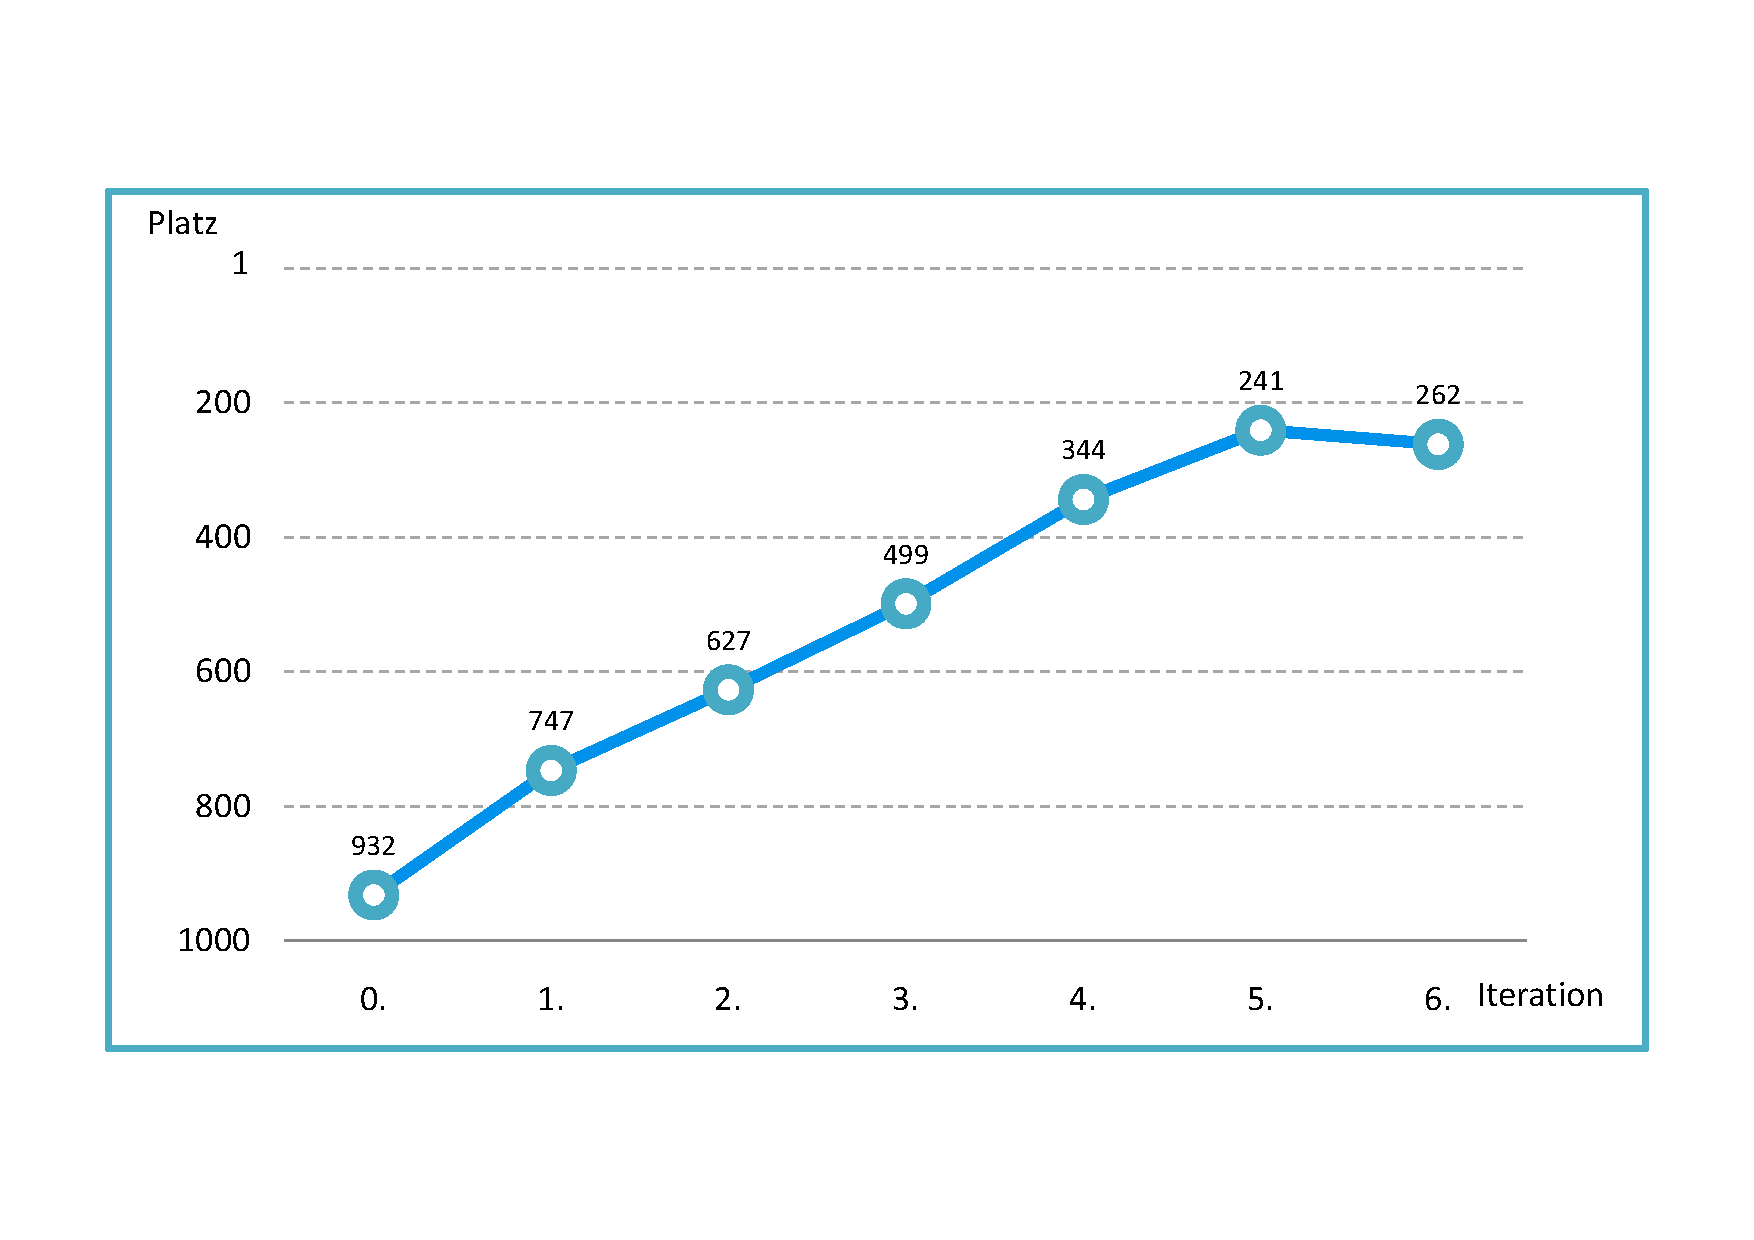
\includegraphics[width=0.85\linewidth]{Bilder/Trenddiagramm_Platzierungen}
\caption{Trenddiagramm unserer Kaggle-Platzierung}
\label{fig:Trenddiagramm_Platzierungen}
\end{figure}

Wie im Diagramm zu sehen, konnte mit den ersten fünf Iterationen die Qualität der Vorhersage verbessert werden. In Iteration 4 konnten wir das Ergebnis der Gruppe aus dem Vorjahr übertreffen und haben letztendlich mit Iteration 5 unsere bisher beste Platzierung erreicht.

Die Auswahl eines Projektes auf der Plattform Kaggle.com hatte für uns den besonderen Vorteil, dass wir unsere Ergebnisse direkt bewerten lassen konnten, auch wenn der Wettbewerb bereits beendet war. So konnte nach jeder Änderung geprüft werden, ob die Vorhersage verbessert wurde oder nicht. Zudem bestand die Möglichkeit, sich mit Data-Mining-Experten zu messen.

Generell gibt die Veranstaltung einen guten Einstieg in Big-Data und die vorhandenen Werkzeuge. Wir als Gruppe sind mit unserem Ergebnis sehr zufrieden, aber es bleibt die Erkenntnis, dass es ein sehr umfassendes Gebiet ist, so dass für ein erfolgreiches Arbeiten in dem Bereich mehr als eine Veranstaltung notwendig ist.
